\documentclass{standalone}
\usepackage{graphicx,float}
\usepackage{tikz}
\usetikzlibrary{shapes,snakes,arrows,chains}
\usetikzlibrary[calc]
\begin{document}
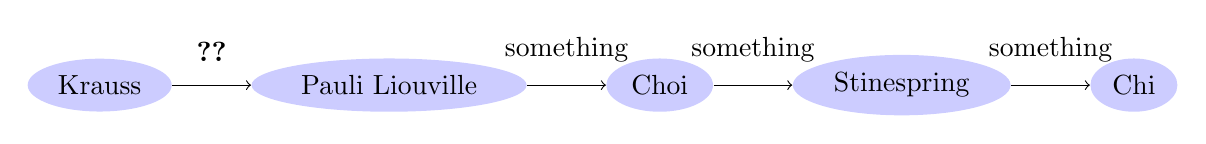
\begin{tikzpicture}[node distance=1cm,auto]
\node[ellipse, fill=blue!20] (p1) {Krauss};
\node[ellipse, right= of p1, fill=blue!20] (p2) {Pauli Liouville};
\node[ellipse, right= of p2, fill=blue!20] (p3) {Choi};
\node[ellipse, right= of p3, fill=blue!20] (p4) {Stinespring};
\node[ellipse, right= of p4, fill=blue!20] (p5) {Chi};
\path[draw,->] (p1) --node[above=0.5em]{\ref{krauss_process}} (p2);
\path[draw,->] (p2) --node[above=0.5em]{something} (p3);
\path[draw,->] (p3) --node[above=0.5em]{something} (p4);
\path[draw,->] (p4) --node[above=0.5em]{something} (p5);
\end{tikzpicture}
\end{document}